% !TEX root = ../my-thesis.tex
%
\chapter{Background}
This section will provide the reader with the required knowledge to understand the attack presented in this paper. First we will introduce the basic concepts of identification and signature schemes, then we will discuss the mathematical concepts of lattices and the computational problems lattice-based cryptography is based upon. Finally we will provide brief information about fault attacks in general.

\section{Identification and signature schemes}
In the public key setting signature schemes are constructions which allow to digitally sign messages. Messages can be can be anything that can be represented with zeroes and ones, e.g. PDF-files, software, videos and photos.

Just like analog signatures digital signatures have the property that they can be efficiently created, that they are valid just for a specific message, that everyone else can verify if a message-signature pair is authentic and that the signer is not able to deny a signature which is valid.

Formally Katz and Lindell \cite[p.~442]{katzlindell} describe a signature scheme as follows:

\begin{definition}[Signature Scheme]
A \textnormal{(digital) signature scheme} consists of three probabilistic polynomial-time algorithms \textnormal{(Gen, Sign, Vrfy)} such that:
\begin{enumerate}
    \item The \textnormal{key generation algorithm Gen} takes as input a security parameter $1^n$ and outputs a pair of keys (pk, sk). These are called the \textnormal{public key} and \textnormal{private key}, respectively. We assume that pk and sk each has length at least $n$. and that $n$ can be determined from pk or sk.
    
    \item The \textnormal{Sign algorithm} takes as input a private key sk and a message $m$ from some message space (that may depend on pk). It outputs a signature $\sigma$, and we write this as $\sigma \leftarrow \textnormal{Sign}_{\textit{sk}}(m)$. 
    
    \item The determininistic \textnormal{verification algorithm Vrfy} takes as input a public key pk, a message $m$, and a signature $\sigma$. It outputs a bit $b$, with $b = 1$ meaning \textnormal{valid} and $b = 0$ meaning \textnormal{invalid}. We write this as $b := \textnormal{Vrfy}_{\textit{pk}(m, \sigma)}$.
\end{enumerate}
It is required that except with negligible probability over (pk, sk) output by $\textnormal{}{Gen}(1^n)$, it holds that $\text{Vrfy}_{\textit{pk}}(m, \text{Sign}_{\textit{sk}}(m)) = 1$ for every (legal) message $m$.

If there is a function $l$ such that for every (pk, sk) output by $\text{Gen}(1^n)$ the message space is $\{0,1\}^{l(n)}$, then we say that \textnormal{(Gen, Sign, Vrfy)} is a \textnormal{signature scheme for messages of length $l(n)$}.
\end{definition}





\section{Lattices}
The general definition of a lattice is as follows:
\begin{definition}[Lattice]
A $n$-dimensional lattice $Λ$ is a discrete subgroup of $\mathds{R}^n$.
\end{definition}

Lattices are often defined by $k$ linearly independent basis vectors $b_1, \ldots, b_k \in \mathds{R}^n$.
Given these basis vectors, the corresponding lattice $Λ(b_1, \ldots, b_k)$ is defined as $Λ(b_1, \ldots, b_k) =  \{\sum_{i = 1}^k a_i b_i \vert a_i \in \mathds{Z}\}$.
In cryptography the lattices of interest are mostly discrete subgroups of $\mathds{Z}^n$ or $\mathds{Z}_q^n$ and in practice most modern lattice based cryptographic lattice primitives use so called ideal lattices. These kind of lattices were first introduced by Lyubashevsky and Micciancio \cite[p.~149]{idealdef} and they define them as follows:

\begin{definition}[Ideal Lattice]
An ideal lattice is an integer lattice $Λ(b_1, \ldots, b_k) \subseteq \mathds{Z}_n$ with $b_1, \ldots, b_k \in \mathds{Z}_q$ being the basis vectors of that lattice, such that $Λ(b_1, \ldots, b_k) = \{g \bmod f \vert g \in I\}$ for some monic polynomial $f$ of degree $n$ and ideal $I \subseteq \mathds{Z}[x]/(f)$.
\end{definition}

These ideal lattices have the great advantage that they can reduce public and private key sizes and, if proper parameters are chosen, the ring operations (multiplying polynomials) can be performed very efficiently using the number theoretic transform (NTT) \cite{ntt} speeding up the computations significantly. While the general definition of ideal lattice is hard to grasp, in this thesis we will only deal with the ideal lattice of the form $\mathds{Z}[x]/(x^n + 1)$. These kind of lattices have the additional property that they are nega-cyclic, meaning that if the vector $(a_1, a_2, \ldots, a_{n-1}, a_n)$ is in in the lattice, the rotated and negated vector $(-a_n, a_1, \ldots, a_{n-2}, a_{n-1})$ is also in the lattice \cite[p.~166]{negadesc}.


Next we introduce two basic properties of lattices which are often of great interest:

\begin{definition}[Shortest Vector]
A shortest vector of a lattice $Λ$ according to a norm $\norm{\cdot}$ is a nonzero lattice vector $v \in Λ \setminus \{0\}$ such that for all $w \in Λ \setminus \{0\}$ it holds that $\norm{v} \leq \norm{w}$.
\end{definition}

\begin{definition}[Closest Vector]
Given a $n$-dimensional lattice $Λ$ and a point $p \in \mathds{R}^n$ and a norm $\norm{\cdot}$
a closest vector to the point $p$ is a vector $v \in Λ$ such that for all $w \in Λ$ it holds that $\norm{p - v} \leq \norm{p - w}$.
\end{definition}


%\subsection{Closest Vector to a point $w \in \mathds{R}^n$}
%The closest vector to a point $w \in \mathds{R}^n$ is a vector $v \in Λ$ which is, according to a metric to a metric, closest to $v$.


\subsection{Lattice Problems}
Lattice problems are problems which are related to lattices. Such problems are used to build lattice-based cryptographic primitives.
The Closest Vector Problem (CVP) and the Shortest Vector Problem (SVP) are the fundamental problems of lattice based cryptography as they have been well studied and they appear to be resistant against quantum computers. They are defined as follows:

\begin{definition}[Shortest Vector Problem (SVP)]
Given $k$ basis vectors $b_1, \ldots, b_k \in \mathds{R}^n$ which define the lattice $Λ(b_1, \ldots, b_k)$, find a shortest vector in $Λ(b_1, \ldots, b_k)$.
\end{definition}

\begin{definition}[Closest Vector Problem (CVP)]
Given $k$ basis vectors $b_1, \ldots, b_k \in \mathds{R}^n$ which define the lattice $Λ(b_1, \ldots, b_k)$ and a point $p \in \mathds{R}^n$, find a closest vector $v \in Λ(b_1, \ldots, b_k)$ which is closest to $p$.
\end{definition}

In lattice-based cryptography new problems which are developed to build a basis for new cryptographic schemes often prove their hardness by reduction, i.e. showing that if one can solve the new problem, one can also solve CVP or SVP.

Using such reductions, the entire lattice based cryptography is based on solid foundations.

\subsubsection{Short Integer Solutions Problem}
The Short Integer Solution (SIS) problem was first introduced Ajtai in 1996 \cite{sis}.
It is defined as follows:
\begin{definition}[Short Integer Solution (SIS)]
Let $A \in \mathds{Z}_q^{m \times n}$ chosen uniformly at random. According to a norm $\norm{\cdot}$, find a vector $x \in \mathds{Z}_q^n$ such that $Ax = 0$ and $\lvert \lvert x \rvert \rvert$ is small and non-trivial.
\end{definition}

Ajtai showed in his work \cite{sis}  that that if one is able to solve the SIS problem with probability at least $\frac{1}{2}$ one can solve SVP with a probability near 1. Thus the SIS problem is at least as hard as SVP. The SIS problem is used by many latticed-based cryptographic schemes to prove their security.






\subsubsection{Ring-LWE and the Module-Ring-LWE}
The  Learning with Errors over Rings problem, also referred as search-RLWE and the generalized variant which is known as Module-LWE or Ring-Module-LWE form the foundations for many lattice based signature and key encapsulation schemes.

Here we will give a more concrete definitions than the original ones \cite{rlwe,glwe} which will be just as general enough to cover all signature schemes we will discuss here.

First we will describe the ring we will be working with:
Let $n$ be a power of two. Let $q$ be an odd prime. Let $\mathds{Z}_q$ be the ring of integers modulo $q$. Then we define the ring $\mathcal{R}_q = \mathds{Z}_q[x]/(x^n+1)$.
 
 Next both problems require some sort of error distribution $\chi$. We will either use the discrete gaussian distribution centered at zero with standard derivation $σ$ or %a uniform one, centered at zero.
 a uniform distribution over a integer range, e.g. $[-(2^{21} - 1), 2^{21} - 1] \cap \mathds{Z}$.
 
 The search variant of the Ring-LWE problem is defined as follows:
 \begin{definition}[Ring-LWE]
 For a given $s \in \mathcal{R}_q$, given pairs of the form $(a_i, b_i = a_i \cdot s + e_i) \in \mathcal{R}_q \times \mathcal{R}_q$, where $a_i \in \mathcal{R}_q$ with coefficients uniformly at random and $e_i$ chosen according to $\chi$, find $s$.
 \end{definition}
 
 The Module-Ring-LWE problem can be seen as an generalization of the Ring-LWE problem:
\begin{definition}[Module-Ring-LWE]
For a given $\bm{s} \in \mathcal{R}_q^k$, given pairs of the form $(\bm{a}_i, b_i = \langle \bm{a}_i, \bm{s} \rangle + e_i) \in \mathcal{R}_q^k \times \mathcal{R}_q^k$, where $\bm{a}_i \in \mathcal{R}_q^k$ with polynomials with coefficients uniformly at random and $e_i$ chosen according to $\chi$, find $\bm{s}$.
\end{definition}

We can see that for $k = 1$ the Module-Ring-LWE problem is the same as the Ring-LWE problem.

\section{Fiat-Shamir with aborts}
Fiat-Shamir with aborts describes a lattice based identification scheme as well as a lattice-based signature scheme, first introduced by Lyubashevsky \cite{fiatshamirabort}.   This identification scheme uses a provable collision resistant lattice-based hash function. Based on this identification scheme Lyubashevsky used the Fiat-Shamir heuristic \cite{fiatshamir} to construct a lattice-based signature scheme. The general design is used by many more recent lattice-based signature schemes such ass BLISS, Dilithium as well as qTESLA.


The Fiat-Shamir with aborts identification scheme has the general structure of a sigma-protocol: First the prover commits to a value, the commitment value, then the challenger sends a value, the so called challenge, to the prover. The prover then performs an operation using the commitment value, challenge and secret key which proves the challenger that he indeed possesses the secret key. The novelty the Fiat-Shamir with aborts scheme is that the prover may abort the identification process. In this case nothing is proven to the challenger.

The aborts allow the scheme to use smaller masking values which reduces signature size while still keeping the scheme secure.

Both, the identification scheme as well as the signature scheme, can work over the ring $\mathcal{R}_q = \mathds{Z}_q[x] / (x^n + 1)$ and require a linear collision resistant hash function $h: \mathcal{R}_q^m \mapsto \mathcal{R}_q$ from a set $\mathcal{H}$ of collision resistant hash functions.

\subsection{The identification scheme}
The private key of the prover is a vector $\bm{s} \in D_s^m$ from a secret key domain $D_s$.
The public key is the hash function $h \in H$ as well as $S = h(\bm{s})$.

The commitment value is calculated by choosing a random $\bm{y} \in D_y^m$ from a commitment domain and calculating $Y = h(\bm{y})$.
Next the challenger chooses an $c \in D_c$ from a challenge domain $D_c$. The prover then computes $\bm{z} = \bm{s}c + \bm{y}$, aborts if $\bm{z}$ is not in a good range, i.e. $\bm{z} \notin G^m$, and otherwise sends $\bm{z}$ to the challenger.

The verifier accepts if $\bm{z} \in G^m$ and $h(\bm{z}) = Sc+Y$. The scheme is correct because $h(\bm{z})= h(\bm{s} c) + h(\bm{y}) = h(\bm{s}) c + h(y) =Sc+Y$.

This identification scheme is considered secure as it is proven that if an attacker can break the scheme he can also break an approximated version of SVP.

\subsection{The signature scheme}
The signature scheme is similar to the identification scheme. It differs from the identification scheme mainly in that it additionally requires a random oracle $H$ and that the challenge $c$ is replaced by $e = c = H(h(\bm{y},\mu))$, where $μ$ is the message. Replacing the challenge with the random oracle removes the needed interaction between the two parties. In detail the signature scheme is described in Figure \ref{fig:abortsig}. The scheme is correct because $H(h(\bm{z}) - Sc, \mu) = H(h(\bm{s} c + \bm{y}) - Sc, \mu) = H(S c + Y - Sc, \mu) = H(Y, \mu)$.

\begin{figure}[h]
\centering
\fbox{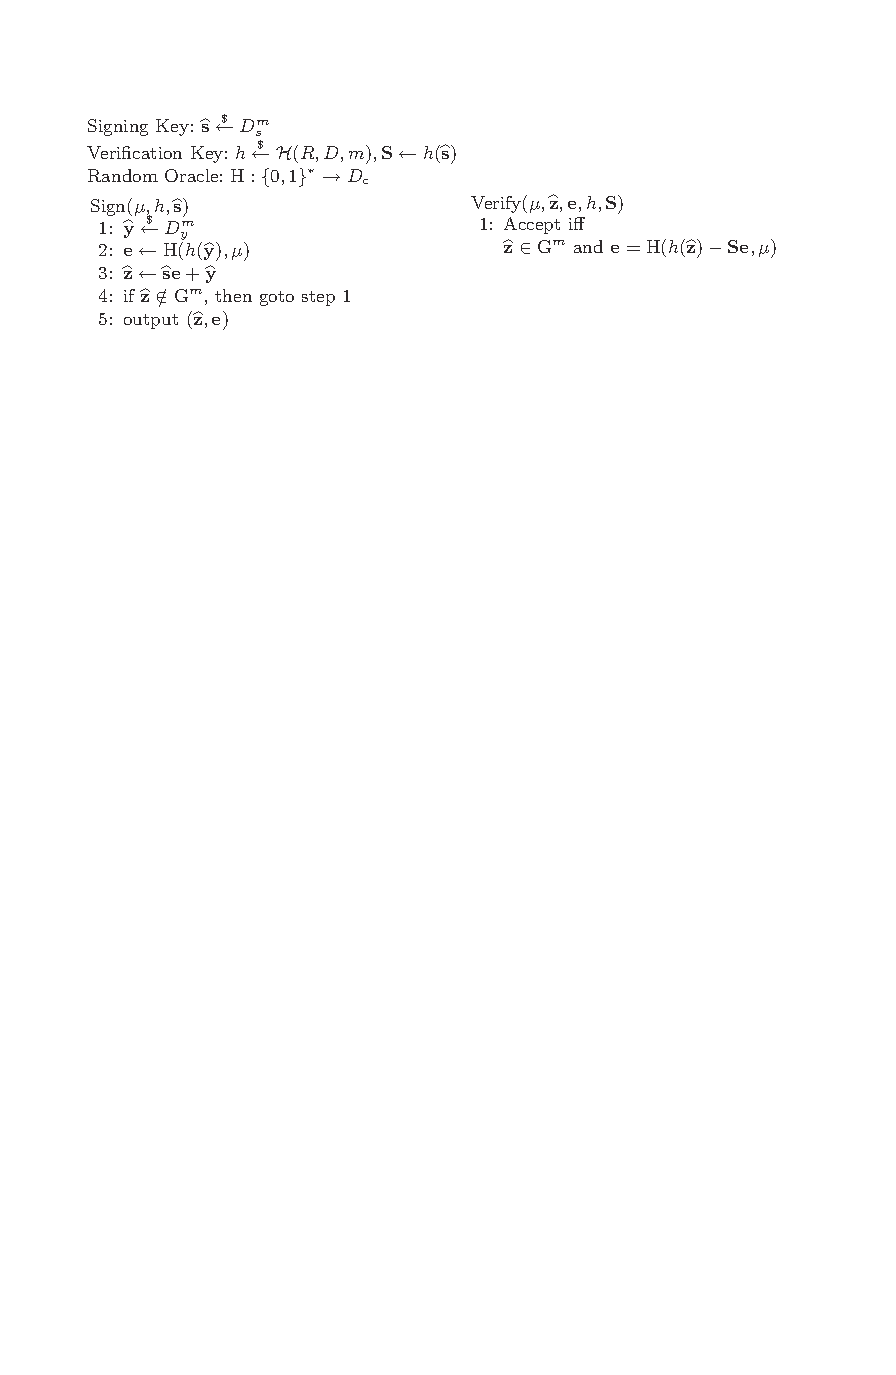
\includegraphics[width=.99\linewidth,trim=40 500 55 54,clip]{plots/loopabortsig}}
\caption{The Fiat-Shamir with aborts signature scheme. Figure copied from \cite[p.~611]{fiatshamirabort}.}
\label{fig:abortsig}
\end{figure}

\section{Lattice based signature schemes}
In this section we will briefly explain the how the signature schemes we will attack work. For each signature we will explain the key generation, the signature generation and the signature verification.
%\todo{write something here}
\subsection{Dilithium}
\label{sec:explaindilith}
Dilithium is currently the only PQC signature scheme that is both recommended and to be standardized by the NIST. \cite{niststatus} The authors proposed parameter sets for the NIST security levels 2, 3 and 5 \cite[pp.~16--17]{dilithium_spec}.

The signature works over the ring $\mathcal{R}_q = \mathds{Z}_q[x]/(x^n+1)$ where $q$ is an odd prime. Simplified works as follows:
\begin{itemize}
    \item \textbf{Key generation} First a $k \times l$ matrix $\bm{A}$ of polynomials with uniform coefficients in $\mathds{Z}_q$ is sampled as well as two secret vectors $(\bm{s}_1, \bm{s}_2) \in S_\eta^l \times S_\eta^l$. $S_\eta^k$ and $S_\eta^l$ denote the set of vectors of polynomials with coefficients with absolute value no more than $\eta$ with $k$ or $l$ entries respectively.
    Then the vector $\bm{t} = \bm{A}\bm{s}_1 + \bm{s}_2$ is calculated.
    Finally the public key is the pair $(\bm{A}, \bm{t})$ and the private key is the tuple $(\bm{A}, \bm{t}, \bm{s}_2, \bm{s}_2)$.
    
    \item \textbf{Signature generation}
    First the vector $\bm{y} \in \tilde{S}_{\gamma_1}^l$ is sampled. The only difference between $\tilde{S}_{\gamma_1}^l$ and $S_{\gamma_1}^l$ is that $\tilde{S}_{\gamma_1}^l$ does not contain any polynomial with coefficient $-\gamma_1$.
    Then the high bits of $\bm{w}_1 = \bm{A}\bm{y}$ together with the message $M$ are hashed to the ball $B_\tau$. The Ball $B_\tau$ is the set of polynomials with exactly $\tau$ coefficients being $-1$ or $1$ and the rest zero. The output of the hash function is the commitment value (commitment polynomial) $c$.
    Finally the vector $\bm{z} = \bm{y} + c \bm{s_1}$ is calculated. If $\bm{z}$ passes a tests which ensures that no information about the secret polynomials is leaked, the signature defined as the pair $\sigma = (\bm{z}, c)$ is outputted. Otherwise the process will be repeated until a generated signature passes the tests and can be outputted.
    
    \item \textbf{Verification}
    To verify a signature $\sigma$ of a message $M$ according to a public key \textit{pk} the high bits of $\bm{w}_1 = \bm{A} \bm{z} - c \bm{t}$ are calculated, we name them $\bm{w}_1'$. Then the signature is accepted iff $\norm{\bm{z}}_\infty \leq \gamma_1 - \beta$ and $c = H(M \Vert \bm{w}_1')$.
\end{itemize}
This simplified version of the Dilithium signature scheme is also depicted in Algorithm \ref{alg:dilithium}.

To see why the scheme is correct the interesting part is the second condition which is checked. The question is whether following holds:
\begin{align}
\label{dilithium_correct}
	c = H(M \Vert \bm{w}_1') = H(M \Vert \text{HighBits}(\bm{A}\bm{y}))  \overset{?}{=}  H(M \Vert \text{HighBits}(\bm{A} \bm{z} - c \bm{t}))
\end{align}
We know that
\begin{align}
	\bm{A} \bm{z} - c \bm{t} = \bm{A}\bm{y}+c\bm{A}\bm{s}_1 - c\bm{A}\bm{s}_1 - c \bm{s}_2 = \bm{A}\bm{y}- c \bm{s}_2
\end{align}
Per definition of the $c$ and $\bm{s}_2$ the coefficients of  $c \bm{s}_2$ can be at most $β$. Because $β$ is comparatively small this addition / subtraction does not affect the high bits of  $\bm{A}\bm{y}$. Thus the equation \eqref{dilithium_correct} holds and the signature scheme is correct.

The security of the scheme is based on the hardness of the Module-LWE problem as well as the SIS problem.

The actual scheme contains many improvements to decrease the memory footprint, decrease execution time and the amount of entropy required but these details are not required for understanding our fault attack nor do they affect our attack.

\begin{algorithm}
\SetKwProg{Fn}{Function}{ is}{end}


\SetKwFunction{Gen}{Gen}
\SetKwFunction{Sign}{Sign}
\SetKwFunction{Verify}{Verify}

\SetKwFunction{HighBits}{HighBits}
\SetKwFunction{LowBits}{LowBits}

\Fn{\Gen{}}{
		$\bm{A} \gets R_q^{k \times l}$\;
		$(\bm{s}_1, \bm{s}_2) \gets S_{\eta}^l \times S_{\eta}^k$\;
		$\bm{t} \gets \bm{A} \bm{s}_1 + \bm{s}_2$\;
		\Return (\ArgSty{pk} $= (\bm{A}, \bm{t})$, \ArgSty{sk} $= (\bm{A}, \bm{t}, \bm{s}_1, \bm{s}_2)$)\; 
}

\SetKwFunction{H}{H}
\Fn{\Sign{sk $= (\bm{A}, \bm{t}, \bm{s}_1, \bm{s}_2)$, M}}{
		$\bm{z} \gets \bot$\;
		\While{$\bm{z} = \bot$}{
			$\bm{y} \gets \widetilde{S}^{l}_{\gamma_1}$\;
			$\bm{w}_1 \gets$ \HighBits{$\bm{Ay}, 2 \gamma_2$}\;
			$c \in B_{\tau} \gets$ \H($M \Vert \bm{w}_1$)\;
			$\bm{z} \gets \bm{y} + c \bm{s}_1$\;
			\If{$\norm{\bm{z}}_\infty \geq \gamma_1-\beta$ or \LowBits{$\bm{A}\bm{y} - c \bm{s}_2$} $\geq γ_2 - β$}{
				$\bm{z} \gets \bot$\;
			}
		}
		\Return $σ = (\bm{z}, c)$
}

\Fn{\Verify{pk $= (\bm{A}, \bm{t})$, M, $σ = (\bm{z}, c)$}}{
	$\bm{w}_1' \gets$ \HighBits{$\bm{A}\bm{z}$, $2γ_2$}\;
	\eIf{$\norm{\bm{z}}_\infty < γ_1 - β$ and $c =$ \H{$M \Vert \bm{w}_1'$}}{
		Accept
	}{
		Reject
	}
}


\caption{Simplified Dilithium signature scheme.}
\label{alg:dilithium}
\end{algorithm}

\subsection{qTESLA}
The qTESLA signature scheme \cite{qtesla} was selected for the second round of the NIST post-quantum cryptography standardization project but was not selected for round three.
When describing the scheme we will leave out various checks which are performed during key generation, signature generation and verification and also some implementation details. The checks include the rejection sampling
but also various checks which aim to counteract fault attacks. None of these checks detect our fault attack because our attack produces perfectly valid signatures. For the reader interested in all details of this signature scheme we refer to \cite{qtesla}.

\subsubsection{Notation}
qTESLA uses the ring, $\mathcal{R}_{q} = \mathds{Z}_{q}[x] / (x^{n} + 1)$ with $n \in \{1024, 2048\}$ and $q$ an odd prime. The set $\mathcal{R}_{[B]} \subseteq \mathcal{R}_q$ is defined as $\mathcal{R}_{[B]} = \{\sum_{i=0}^{n-1}f_{i}x^{i} \in \mathcal{R} \vert f_{i} \in [-B, B]\}$ and the set $\mathds{H} \subseteq \mathcal{R}_q$ is defined as $\mathds{H} = \{\sum_{i=0}^{n-1}f_{i}x^{i} \in \mathcal{R} \vert f_{i} \in \{-1, 0, 1\}, \sum_{i=0}^{n-1}f_{i} = h\}$, $h \in {25, 40}$. The $[\cdot]_M$ operator rounds aways the last few bits of its argument, roughly speaking. $G$ and $H$ are hash functions. $H$ applies the rounding operation $[\cdot]_M$ to any polynomials from $\mathcal{R}_q$ it receives as input.

\subsubsection{Key generation}
From an initial so called \say{pre-seed}, a $κ$ bit long uniform random bitstring, multiple different seeds like $\textbf{seed}_{y}$ and  $\textbf{seed}_{a}$ are generated to be used to sample the following polynomials.
First the public key polynomials $a_{1}, \ldots, a_{k}$ are sampled uniformly from $\mathcal{R}_{q}$ using $\textbf{seed}_{a}$.
Next the secret polynomial $s \in \mathcal{R}_q$ is sampled with coefficients distributed following the discrete Gaussian distribution with standard deviation $\sigma$.
The error polynomials $e_{1}, \ldots, e_{k} \in \mathcal{R}_q$ are sampled just like $s$ was sampled previously.
The public key polynomials $t_{i}$ are then calculated as $t_{i} = a_{i} s + e_{i}$ for $i \in {1, \ldots, k}$.
Finally the value $g$ is crafted by hashing all public key polynomials $t_{i}$ using $H$.
The secret key is then the tuple $(s, e_{i}, \ldots, e_{k}, \textbf{seed}_{a},  \textbf{seed}_{y}, g)$ and the public key is $(t_{1}, \ldots, t_{k},  \textbf{seed}_{a})$.

\subsubsection{Signature generation}
When signing a message $m$, first a randomness $r$ is collected. Based on this randomness the masking polynomial $y$ is sampled uniformly from $\mathcal{R}[B]$.
Next the polynomials $v_{i} = a_{i}y$ are calculated for $i \in \{1, \ldots, k\}$. These polynomials are then hashed together with $G(m)$ and $g$. This hash is then used to construct the commitment polynomial $c \in \mathds{H}$. Finally the $z = y + sc$ is calculated and the signature is defined as the pair $(z, c)$.

\subsubsection{Signature verification}
Given the public key, private key, a signature $(z, c)$ and the message $m$, to verify a signature we first calculate $w_{i} \leftarrow a_{i} z - t_{i} c$.
The signature is valid iff $z \in \mathcal{R}_{[B-S]}$ and $c = H(w_{1}, \ldots, w_{k}, G(m), G(t_{1}, \ldots, t_{k}))$.
The second condition holds for valid signatures because \cite[p. 445]{qtesla}:
% TODO: understand why []_{M} is used then it is not used in the alg? 
\begin{align}
	[w_i]_{M} = [a_{i}z-t_{i}c]_{M} = [a_{i}(y+sc) - (a_{i}s+e_{i})c]_{M} = [a_{i}y - e_{i} c]_{M} = [a_{i}y]_{M}
\end{align}
Note that the last equations holds because $e_ic$ only has small coefficients, thus only affecting the lower bits of $a_iy$, and $[\cdot]_{M}$ rounds away these lower bits.



\subsection{BLISS}
\label{sec:blissdesc}
BLISS \cite{bliss}  is an acronym for \say{Bimodal Lattice Signature Scheme}. It introduced a new more efficient way of rejection sampling by using a bimodal Gaussian distribution instead of a Gaussian one. We will skip some technical details parts of the signature scheme they are not relevant for our attack.

\subsubsection{Key generation}
\label{sec:blisskeygen}
First the two polynomials $f$ and $g$ are sampled with $\lfloor \delta_{1} n \rfloor$ coefficients uniformly from $\{-1, 1\}$ and   $\lfloor \delta_{2} n \rfloor$ coefficients uniformly from $\{-2, 2\}$, rest zero.
The private key $\bm{S}$ is now defined as $\bm{S} = (s_{1}, s_{2})^{t} = (f, 2g+1)^{t}$.
For the public key we first calculate $a_{q} = (2 g + 1) / f \bmod q$ and set $\bm{A} = (2 a_{q}, q - 2) \bmod 2q$.

If a check (which we did not mention here) on $S$ does not pass or $f$ is not invertible the key generation restarts until it succeeds. Once it succeeded, due to the way they keys were constructed, it holds that $\bm{A}\bm{S} = q \mod 2q$.

\subsubsection{Signature generation}
The signature generation begins by sampling two masking polynomials $y_{1}$ and $y_{2}$ with coefficients from the the discrete Gaussian distribution $D_{\sigma}$.
Then we calculate $u = \zeta a_{1} y_{1} + y_{2} \bmod 2q$ and the commitment polynomial $c = H({\lfloor u \rceil}_{d} \bmod p, \mu)$.
Here $H$ is a cryptographically secure hash function mapping to polynomials with exactly $\kappa$ coefficients in $\{-1, 1\}$and the rest zero.
Finally $z_{1}$ and $z_{2}$ are calculated by first sampling $b \in \{0,1\}$ and then calculating $z_{1} = y_{1} + (-1)^{b} s_{1}c$ and $z_{2}$ analogously:  $z_{2} \leftarrow y_{2} + (-1)^{b} s_{2}c$.
Now the rejection step is performed. Finally let $z_2^\dagger = (\lfloor u \rceil_d - \lfloor u - z_2\rceil_d) \bmod p$.
The signature is the triple $(z_{1}, z^{\dagger}_{2}, c)$.

\subsubsection{Signature verification}
% TODO: how does this work ...

%This does not make any sense. I do not understand why this signature scheme is correct \ldots
%\begin{align}
%	\zeta a_{1} z_{1} + \zeta q c &= \zeta a_{1} (y_{1} + (-1)^{b} s_{1}c) + \zeta q c \
%	&=  \zeta a_{1} y_{1} +  \zeta a_{1} (-1)^{b} s_{1}c + \zeta q c \
%	&\overset{\bm{a}_{1} \bm{s}_{1} = \bm{a}_{1} (- \bm{s}_{1})}{=}   \zeta a_{1} y_{1}+  \zeta a_{1} s_{1}c + \zeta q c \
%	&\overset{\bm{a}_{1} \bm{s}_{1} = 1}{=}   \zeta a_{1} y_{1}+  \zeta 1 c + \zeta q c \
%	&=   \zeta a_{1} y_{1}
%\end{align}
To verify a signature $(z_1, z_2^\dagger, c)$ given a public key $\bm{A} = (a_1, q - 2)$ the verifier first checks whether $\norm{(z_1 \vert 2^d \cdot {z_2}^\dagger)}_2 > B_2$ or
$\norm{(z_1 \vert 2^d \cdot {z_2}^\dagger)}_\infty > B_\infty$ holds.
If so he rejects the signature. Finally he accepts the signature iff $c = H(\lfloor ζ a_1 z_1 + ζ q c\rceil_d + z_2^\dagger \mod p, μ)$.
 
 Understanding why the signature verification is correct is not straight-forward for BLISS. Because this aspect is irrelevant for the understanding of our attack and for the sake of brevity we will refer the interested reader to the original publication  \cite{bliss_full} for details.  \todo{if time, take a look how this works}
% \todo{Why is this correct? I do not understand this, too complicated for me ...}





\section{Fault attacks}
Fault attacks describe an attack model where the attacker is able to choose the physical environment of a device under attack (DUA). The attacker tries to cause the device to malfunction and thus to output the result of a faulty calculation. When the device is running a cryptographic algorithm like an encryption algorithm or signature algorithm a faulty output like a faulty ciphertext or a faulty signature may reveal information about the internal state of the device which may include information of the secret key.

The idea of a fault attack was first introduced in \cite{bellcore} which is now commonly known as the bellcore attack. The bellcore attack is able to break RSA-CRT with a single faulty signature. DES and AES can be broken with two faulty ciphertexts \cite[p.~544]{fault_survey}. This shows how powerful the fault attack model is.

Faults can be achieved in different ways. In a voltage-glitch attack the supply voltage of the DUA is increased or decreased for a short amount of time to a range the device is not rated for, thus causing unexpected, faulty behaviour.
A clock-glitch describes an attack, where the clock signal is disturbed. An attacker could for a single clock cycle significantly reduce the time the clock signal is high. This may result in the processor to skip an instruction. If the skipped instruction would have prevented a loop from aborting, this could be called loop-abort attack. This type of fault attack has already been shown to work on lattice-based signature schemes by Espitau et al. \cite[pp.~1545--1546]{espitau_kem}.
Shining light on the DUA can also cause a fault. The light can be a flash or laser. Because the light needs to be applied directly to the silicone this attack is semi-invasive as the plastic layer has to be removed \cite[pp.~161--162]{older_fault_survey}.
Fault attacks are also possible by creating an electromagnetic field close to the circuit. Such attacks work even without opening the package of the IC \cite{fault_magnetic}. 
Further types of attacks exists, see \cite{fault_survey} for a survey.


For many of the attacks countermeasures do exists and are used in practice. Countermeasures can either be implemented in hardware (e.g. detect high / low voltage) or in software (e.g. check if a previous calculation seems plausible).
Because this attack model gives the attacker seemingly endless possibilities to attack it is very hard to defend against.
%\todo{Add more details, especially to loop-abort attacks and example of loop-abort in practice}

